\section{Generate triplets \er{NO\_GenTripl}}

The goal here is to build a set of optimal triplet pairs from the existing relative orientations. As is illustrated schematically in Fig.~\ref{fig:workf1GenTrip} the  \er{TestLib NO\_GenTripl} launches \er{GenTriplet\_main} (see Alg.~\ref{alg:GenTriplMain}) for a pattern of images. Then, for each edge of the epipolar graph, the Alg.~\ref{alg:GenTriplArc} is called. 

\begin{figure}[h!]
\centering
\begin{tikzpicture} 
\node (start) at (10,0) [call] {TestLib NO\_GenTripl}; 
\node (main) at (0,0) [process] {GenTriplet\_main(), see Alg.~\ref{alg:GenTriplMain}};
 
\node (appli) at (0,-2) [process, text width=7.5cm] {cAppli\_GenTriplet::cAppli\_GenTriplet \\ cAppli\_GenTriplet::GenTriplet() see Alg.~\ref{alg:AppliGenTripl}}; 
\node (GenTri) at (0,-5) [process, text width=8cm] {cAppli\_GenTriplet::GenTriplet(tArcGT $\&$) \\ see Alg.~\ref{alg:GenTriplArc}};


\node (AddSomTmp) at (4.0,-7) [processMul, text width=5cm] {cAppli\_GenTriplet:: AddSomTmp(tSomGT $\&$) see Alg.~\ref{alg:GenTriplAddSom}} ;

\node (InitTri) at (10,-6.75) [processMul, text width=5cm] {if (GetNextSom()) Alg.~\ref{alg:GetNextSom} \\ cGTrip\_AttrSom:: InitTriplet(tSomGT *,tArcGT *) see Alg.~\ref{alg:InitTrip}} ;
\node (AddTrip) at (5.5,-9) [processMul, text width=8cm] {cAppli\_GenTriplet::AddTriplet(tSomGT \&,tSomGT \&,tSomGT \&) \\ see Alg.~\ref{alg:AddTriplet}} ;

\node (GenTria) at (-3,-4.6) {};
\node (GenTrib) at (-2,-4.6) {};
\node (GenTric) at (-1,-4.6) {};
\node (GenTrid) at (1,-4.6) {};
\node (GenTrie) at (2,-4.6) {};
\node (GenTrif) at (3,-4.6) {};

\node (launch3rd) at (-3,-8) {};

\draw [arrow] (start) --  (main); 
\draw [arrow] (main) --  (appli); 

\draw [arrow] (appli) --  node[anchor=west,xshift=-0.5cm] {4} (GenTri);
\draw [arrow] (appli) --  node[anchor=west,xshift=-1.5cm] {1edge} (GenTria);
\draw [arrow] (appli) --  node[anchor=west,xshift=-0.5cm] {2} (GenTrib);
\draw [arrow] (appli) --  node[anchor=west,xshift=-0.5cm] {3} (GenTric);
\draw [arrow] (appli) --  node[anchor=west,xshift=-0.5cm] {5} (GenTrid);
\draw [arrow] (appli) --  node[anchor=west,xshift=-0.5cm] {..} (GenTrie);
\draw [arrow,dashed] (appli) -- node[anchor=west,xshift=-0.5cm] {N} (GenTrif);

\draw [arrow] (GenTri) -- (0,-7) -- (AddSomTmp);
\draw [arrow] (AddSomTmp) -- (InitTri)  ;
\draw [arrow] (GenTri) -- (0,-9) -- (AddTrip);

%\draw [arrow,draw=blue] (launch3rd) -- node[anchor=west,xshift=-4.5cm,yshift=-0.5cm] {\textcolor{blue}{for every "third" image}} (0,-8);
\draw [arrow,draw=blue] (launch3rd) -- (-3,-6.5) --  node[anchor=west,xshift=-4.5cm,yshift=-1.5cm] {\textcolor{blue}{for every "third" image}} (0,-6.5);

\end{tikzpicture}
\caption{The triplet generation workflow. The enumerated arrows launch the GenTriplet method for each edge (i.e. a pair of nodes and the edge connecting them) of the epipolar graph. The methods in purple are launched for each "third" image attached to each edge of the graph.}\label{fig:workf1GenTrip}
\end{figure}

\subsection{Main classes, some typedefs and variables}
\begin{itemize}
\item $cAppli\_GenTriplet$
\item $cGTrip\_AttrSom$ -- class corresponding to a triplet node (its orientation parameters etc)
\item $cGTrip\_AttrASym$ -- ?
\item $cGTrip\_AttrArc$ -- class containing relative rotation corresponding to an edge
\item $cResTriplet$ -- class containing $cXml\_Ori3ImInit$ (xml save)
\item[--] $cTripletInt$ -- typedef to $cTplTriplet<int>$ containing ids of images within a triplet
\item[--] $tSomGT$ -- a node of the graph
\item[--] $tArcGT$ -- an edge of the graph
\item[--] $tGrGT$ -- a graph  
\item[*] $mHautBase$ -- height, used e.g. in the B to H ratio calcul
\item[*] $mMapTriplets$ -- contains all triplets (for each triplet it stores the identifiers of nodes defining the node and the resulting orientations)
\item[*] $mTopoTriplets$ -- contains a list of all accepted triplets (xml of type $Xml_TopoTriplet$)
\item[*] $mTriOfCple$ -- stores edges (i.e. 2 images) and a list of "third" images for each edge 
\item[*] $mVSomVois$ -- a vector of nodes that are neighbouring with an edge in consideration (i.e., they're outside that edge)
\item[*] $mVSomEnCourse$ -- vector of "third" images that are currently connected to an edge
\item[*] $mVSomSelected$ -- vector containing the selected triplets
\end{itemize}

\subsection{Algorithms}

\begin{figure}[H]
\begin{equation}
| C_{2} + \lambda \cdot C_{3} \quad U_{3} \quad U_1 | = 0
\end{equation}\label{eq:coplan}
\begin{equation}
\lambda = -\frac{| C_{2} \quad U_{3} \quad U_1 |}{| C_{3} \quad U_{3} \quad U_1 |}
\end{equation}\label{eq:lambda}
\caption{Computation of orientations of a triplet consistent with relative orientations. See also Alg.~\ref{alg:InitTrip}}
\end{figure}
 

\begin{figure}[H]
\centering
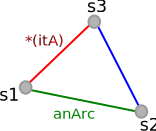
\includegraphics[width=5cm]{img/triplet.pdf}\caption{A triplet defined by 3 nodes and three edges, illustration of the Alg.~\ref{alg:GenTriplArc}. The green edge is the edge entering the $GenTriplet(tArcGT \& anArc)$ method. If s3 exists, there is an edge between s1 and s3. If $(mGrT.edge\_s1s2(anArc.s2(),aS3))$, the blue edge connecting s2 and s3 exists, and therefore a complete triplet is defined.
}\label{fig:triplet}
\end{figure}

\begin{figure}[H]
\centering
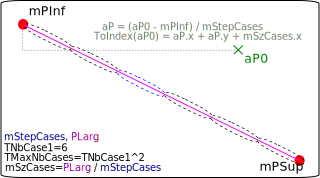
\includegraphics[width=9cm]{img/ToIndex.pdf}\caption{Illustration of the tie-pts indexing method implemented in $ToIndex(const Pt2df \&  aP0)$.}
\end{figure}\label{fig:ToIndex}

%%%%%%%%%%%%%%%%%%%%%%%%%%%%%%%%%%%%%%%%%% GenTriplet\_main
\begin{algorithm}
\caption{\er{$GenTriplet\_main$} def in cNewO\_OldGenTriplets.cpp  }
\begin{algorithmic}
\State 
\\
\Comment \cmt{Initialise the object class}
 \State cAppli\_GenTriplet anAppli(argc,argv);
\\
\Comment {Call the GenTriplet()}
\State anAppli.GenTriplet();

\end{algorithmic}\label{alg:GenTriplMain}
\end{algorithm}


%%%%%%%%%%%%%%%%%%%%%%%%%%%%%%%%%%%%%%%%%% cAppli\_GenTriplet
\begin{algorithm}
\caption{\er{$cAppli\_GenTriplet::cAppli\_GenTriplet$} constructor def in cNewO\_OldGenTriplets.cpp  }
\begin{algorithmic}
\State 
\\
\Comment \cmt{Some member variables}
 \State mVecAllSom - a vector of all nodes
 \State mMapS - a map of graph nodes and the respective image names
 \State mGrT - the epipolar graph
 \State tSubGrGT SubAll \cmt{allows to iterate over a subgraph of edges attached to a node}

 
\\
\Comment \cmt{Initialise the nodes of the graph}
\State mVecAllSom, mMapS
\\
\Comment \cmt{Initialise the edges of the graph}
\For {Each stereo pair}
	\State Get respective nodes from the map of nodes (aS1,aS2)
	\State Get the relative orientation from XML file 
	\State Test the edge from aS1 to aS2  \cmt{?}
	\State Add the edge to the graph mGrT

\EndFor 

\end{algorithmic}\label{alg:AppliGenTripl}
\end{algorithm}



%%%%%%%%%%%%%%%%%%%%%%%%%%%%%%%%%%%%%%%%%% cAppli_GenTriplet::GenTriplet()
\begin{algorithm}
\caption{\er{$cAppli\_GenTriplet::GenTriplet()$} def in cNewO\_OldGenTriplets.cpp  }
\begin{algorithmic}
\State  
\\
\Comment \cmt{Iterate over edges}
\For {All edges between nodes in mVecAllSom}
	 \State Call GenTriplet(*itA);

\EndFor 

\end{algorithmic}\label{alg:GenTripl}
\end{algorithm}

%%%%%%%%%%%%%%%%%%%%%%%%%%%%%%%%%%%%%%%%%% cAppli_GenTriplet::GenTriplet(tArcGT & anArc)
\begin{algorithm}
\caption{\er{$cAppli\_GenTriplet::GenTriplet(tArcGT \& anArc)$} def in cNewO\_OldGenTriplets.cpp  }
\begin{algorithmic}
\State  
\\
\Comment \cmt{Only symmetric edges are dealt with}
\State if (!anArc.attr().IsDirASym() ) return;
\\
\Comment \cmt{Load tie-pts for the stereo pair}
\\
\Comment \cmt{Get the distance between the two most distant points (mPInf,mPSup) in the pair model; return if it is too large}
\State
\\
\Comment \cmt{Some variables}
\State mCurPMed -- median point calculated on all tie-pts of a pair
\State  mCurS1  = $\&$ (anArc.s1());  -- the aS1 in Fig.~\ref{fig:triplet}
\State  mCurS2  = $\&$ (anArc.s2());  -- the aS2 in Fig.~\ref{fig:triplet}
\\
\\
\Comment \cmt{Initialise the triplets. See Fig.~\ref{fig:triplet} for illustration}
\For {all edges attached to mCurS1/aS1}
	 \State Get the second node $(*itA).s2()$ for an edge in consideration and call it aS3 of the triplet
	 \If {there is an edge between aS3 and aS2 of the anArc}
	 	\State call $AddSomTmp(aS3)$, see Alg.~\ref{alg:GenTriplAddSom}  
	 \EndIf

\EndFor 
\\
\\
\Comment \cmt{Iterate over all connected images that are found in mVSomEnCourse and select the "best" ones. The number of selected triplets is defined by $TQuickNbMaxTriplet$ and $TStdNbMaxTriplet$. See Alg.~\ref{alg:GetNextSom}}
\While {aSom = GetNextSom()}
	\State $AddTriplet(*aSom,mCurArc->s1(),mCurArc->s2());$ \cmt{see Alg.~\ref{alg:AddTriplet}}
\EndWhile

\end{algorithmic}\label{alg:GenTriplArc}
\end{algorithm}

%%%%%%%%%%%%%%%%%%%%%%%%%%%%%%%%%%%%%%%%%% cAppli_GenTriplet::AddSomTmp(tSomGT & aS)
\begin{algorithm} 
\caption{\er{$cAppli\_GenTriplet::AddSomTmp(tSomGT \& aS)$} def in cNewO\_OldGenTriplets.cpp  }
\begin{algorithmic}%[1]
\\
\State $mVSomVois.push\_back(\&aS);$
\\
\\
\Comment \cmt{If an approx orientation of triplet is possible, add the "third" image to the current nodes}
\If $InitTriplet$ (\cmt{see Alg.~\ref{alg:InitTrip}})
	\State $mVSomEnCourse.push\_back(\&aS) ;$
\EndIf
\end{algorithmic}\label{alg:GenTriplAddSom}
\end{algorithm}


%%%%%%%%%%%%%%%%%%%%%%%%%%%%% cAppli_GenTriplet::GetNextSom()
\begin{algorithm}
\caption{\er{$cAppli\_GenTriplet::GetNextSom()$}, update the mVSomSelected; def in cNewO\_OldGenTriplets.cpp  }
\begin{algorithmic}
\State 
\\
\Comment \cmt{Leave if your objective is reached, i.e. there are no "third" images in the current nodes or if the number of selected "third" images is already bigger than the $aNbMaxTriplet$}
\State  $if (mVSomEnCourse.empty()) return 0;$
\State  $if (int(mVSomSelected.size()) > aNbMaxTriplet) return 0;$
\\
\\
\Comment \cmt{Get the best GainGlob for all available "third" images and store it in:}
\State aGainMax, aRes, aIndexRes
\\
\Comment \cmt{Remove the best image from mVSomEnCourse}
\State $mVSomEnCourse.erase(mVSomEnCourse.begin()+aIndexRes);$
\\
\Comment \cmt{And save it in the selected images}
\State $mVSomSelected.push_back(aRes);$
\\
\Comment \cmt{Update the cost/gain of the remaining images giventhe best result in $aRes$}
\For {all images in mVSomEnCourse}

	$tSomGT * aSom = mVSomEnCourse[aK];$\\
    $aSom->attr().UpdateCost(aSom,aRes);$ \cmt{see Alg.~\ref{alg:UpdCost}}

\EndFor
\end{algorithmic}
\label{alg:GetNextSom}
\end{algorithm}



%%%%%%%%%%%%%%%%%%%%%%%%%%%%% cGTrip_AttrSom::UpdateCost(tSomGT * aSomThis,tSomGT *aSomSel)
\begin{algorithm}
\caption{\er{$cGTrip_AttrSom::UpdateCost(tSomGT * aSomThis,tSomGT *aSomSel)$}, def in cNewO\_OldGenTriplets.cpp  }
\begin{algorithmic}
\State 
\Comment \cmt{Calculates the new gain as a function of b sur h between aSom and the aSomSel  being the best node}
\State $aNewGain =  mAppli->GainBSurH(aSomThis,aSomSel);$
\\
\\
\Comment \cmt{Get Pds and Dens that will help to define the new global gain/cost}
\State $int * aPdsGlob = mAppli->Pds();$
\State $int * aDens2 = aSomSel->attr().mDens;$
\\
\\
\Comment \cmt{Re-define the gain accordingly:}
\For {All "cases" (here 6*6)}
	\State int aD2 =  aDens2[aK];
    \State ElSetMin(mGain[aK], mDens[aK] * ( aNewGain * aD2 + TQuant*(TQuant-aD2)));
    \State mGainGlob +=  mGain[aK] * aPdsGlob[aK];

\EndFor 

\end{algorithmic}
\label{alg:UpdCost}
\end{algorithm}

 
%%%%%%%%%%%%%%%%%%%%%%%%%%%%%%%%%%%%%%%%%% cGTrip\_AttrSom::InitTriplet(
\begin{algorithm} 
\caption{\er{$cGTrip\_AttrSom::InitTriplet(tSomGT * aSom,tArcGT * anA12)$} def in cNewO\_OldGenTriplets.cpp  }
\begin{algorithmic}%[1]
\State  
\\
\Comment \cmt{Some variables}
\State $anA13$ -- edge from s1 to s3 (\cmt{see Fig.~\ref{fig:triplet}})
\State $anA23$ -- edge from s2 to s3 (\cmt{see Fig.~\ref{fig:triplet}})
\State $aR21$ --  affine rotation (Rot et tr) corresponding to edge between s1 and s2
\State $aR31$ --  affine rotation (Rot et tr) corresponding to edge between s1 and s3
\State $aR31Bis$ -- affine rotation (Rot et tr) corresponding to edge between s1 and s3 \cmt{calculated from aR21 and aR32}
\State $aR32$ --  affine rotation (Rot et tr) corresponding to edge between s2 and s3
\State $aVP1$,$aVP2$,$aVP3$ -- vectors containing tie-pts visible in the triplet
\State $mNb$ -- vector that contains information about tie-pts in an indexed form
\\
\\
\Comment \cmt{Calculate orientations consistent within a triplet (origin in s1) using the known relative orientations. We search for a scale factor $\lambda$ for which the three directions stemming from three images (i.e. nodes) and corresponding to a tie-point will intersect in 3D. We use the coplanarity condition as the mathematical model to calculate it. Its determinant shall be null for the solution to exist. Because we will have as many $\lambda$s as there is tie-points, the final result is the median of all results. Since the multiple points are not really considered in this approach, it will be ill-defined for three colinear perspective center.}
%
\For {all almost tie-pts in $aVP1$ \cmt{(aStep defines the subsample)}}
\\
\\
\Comment \cmt{Get normalised vector directions}
\State $aU31$ -- direction corresponding to tie-pt in s3 calculated from R31
\State $aU2$ -- direction corresponding to tie-pt in s2
\State $aU1$ -- direction corresponding to tie-pt in s1
\State $aU31Bis$ -- direction corresponding to tie-pt in s3 calculated from R31Bis
\\
\State $aVL13$, $aVL23$ are vectors containing all the results calculated using two combinations
\\
\\
\Comment \cmt{Calculate intersection of the points using s1, s2}
\State aPInt12 = InterSeg(aC1,aC1+aU1,aC2,aC2+aU2,OkI);
\\
\\
\Comment \cmt{Impose that s3 is found at the intersection of line s1 s3 and on the bundle stemming from aPInt12 and going towards U31.Save result to aVLByInt}
\State CoordInterSeg(aC1,aC3,aPInt12,aPInt12+aU31,OkI,p,q);
\\
\\
\Comment \cmt{Calculate the perspective center of s3 from aVL13 and aVL23 and aVLByInt}
\State Pt3dr aC31 = aC3 / MedianeSup(aVL13);
\State      Pt3dr aC32 = aC2 + aV3Bis * MedianeSup(aVL23);
\State      mC3 = (aC31 + aC32) / 2.0;
\State      Pt3dr aC3I = aC3 *  MedianeSup(aVLByInt);
\\
\\
\Comment \cmt{The final solution for the perspective center is the one from multiple points (i.e. from the inverse aVLByInt ). As far as the rotation, the avarege result from R31 et R31Bis is taken (orthonormality is imposed with nearest rotation.)}
\State mC3 = aC3I;
\State      mM3 =  NearestRotation((aR31.Mat() + aR31Bis.Mat())*0.5);
\EndFor
\\

\end{algorithmic}
\label{alg:InitTrip}
\end{algorithm}
%%%%%%%%%%%%%%%%%%%%%%%%%%%% CONTINUE 
\begin{algorithm}
\begin{algorithmic}%[40]
\\
\Comment \cmt{Calculate gain and density}
\State $aGain1$, b sur h between s1 and s3
\State $aGain2$, b sur h between s2 and s3
\State $aGain = ElMin(aGain1,aGain2);$
\\
\\
\Comment \cmt{Inside this method, the $mNb$ vector is updated. The size of the vector is equal to $TMaxNbCases$ and it encodes indexed position in an image. To update the $mNb$, each tie-pt is first indexed with ToIndex() (see Fig.~\ref{fig:ToIndex}). The output of the indexing is an int from $0$ to $TMaxNbCases$ and it indicates the position within the $mNb$ vector that will be incremented.}
\State $InitNb(aVP1);$
\\
\\
\\
\Comment \cmt{Using the $mNb$ we now calculate gain scores for each \textit{case element} of the indexed image. The gain depends on points' density in a given \textit{case element}}
\For {all element cases \cmt{i.e. $mSzCases.x*mSzCases.y$, see Fig.~\ref{fig:ToIndex}}}
\State $mDens[aK]$ -- the density per case
\State $mGain[aK]$ -- gain per case
\State $mGainGlob$ -- global gain
\EndFor
\end{algorithmic}
\end{algorithm}


%%%%%%%%%%%%%%%%%%%%%%%%%%%%% cAppli_GenTriplet::AddTriplet
\begin{algorithm}
\caption{\er{$cAppli\_GenTriplet::AddTriplet(tSomGT \&,tSomGT \&,tSomGT \&)$} def in cNewO\_OldGenTriplets.cpp  }
\begin{algorithmic}
 
\State 
\Comment \cmt{Get the corresponding nodes}
\State aA1, aA2, aA3
\\
\\
\Comment \cmt{Normalise the orientations so that the first node has and identity rotation matrix and the bases between the first and the second node is equal to 1. To do that, multiply orientations of nodes aA2 and aA3 by the inverse of aA1; then, divide the orientations by the length of the base between aA1 and aA2.}
\State aR1Inv = aA1.R3().inv();
\State aR1 = aR1Inv*aA1.R3();
\State aR2 = aR1Inv*aA2.R3();
\State aR3 = aR1Inv*aA3.R3();
\State double aD = euclid(aR2.tr());
\State aR2 = ElRotation3D(aR2.tr()/aD,aR2.Mat(),true);
\State aR3 = ElRotation3D(aR3.tr()/aD,aR3.Mat(),true);
\\
\\
\Comment \cmt{Iterate over all (triplet) tie-pts. For each tie-pt in each image get its direction with $AddSegOfRot$. The directions are stored in vectors aW. Intersect the directions in 3D with $InterSeg$. Get the residuals in images, store the mean value in aVRes vector. }
\\
\\
\Comment \cmt{Check if this triplet already exists in the $mMapTriplets$. If it does and the median residual of the current triplet is larger than that of the triplet already stored in the map, it returns from the AddTriplet method. Otherwise it continues.}
\\
\\
\Comment \cmt{Save. Update the $mMapTriplets$, the $mTopoTriplets$ and the $mTriOfCple$.}

\end{algorithmic}\label{alg:AddTriplet}
\end{algorithm}

